\documentclass{beamer}
\usetheme{Darmstadt}
\usecolortheme{orchid}
\usepackage{tikz}
\usetikzlibrary{automata, positioning}
\usepackage{graphics,xcolor}

\newcommand{\nat}{\mathbb{N}}
\newcommand{\ints}{\mathbb{Z}}
\newcommand{\intersection}{\ensuremath{\cap}}
\newcommand{\emptyword}{\ensuremath{\epsilon}}
\newcommand{\len}[1]{\ensuremath{|#1|}}
\newcommand{\union}{\ensuremath{\cup}}
\newcommand{\deltahat}{\ensuremath{\widehat{\delta}}}

\title[Finite-State Automata]{2-way DFA}
\author{xyz}

\begin{document}

\begin{frame}
\frametitle{Outline}
\tableofcontents
\end{frame}

\section{Introduction}

\begin{frame}{What is 2DFA?}
  \begin{block}{2DFA}
    A Two-Way Deterministic Finite Automaton (2DFA) is a type of finite state machine that extends the capabilities of a regular Deterministic Finite Automaton (DFA) by allowing its read head to move \textcolor{red}{bidirectionally} along the input tape. 
   
    
  \end{block}
  \begin{itemize}
    \item 2DFAs were introduced in 1959 by Rabin and Scott.
   \end{itemize}

\end{frame}

\begin{frame}
\frametitle{How 2DFA works?}
%construction of tape to illustrate the working of 2DFA drawing 
\centering
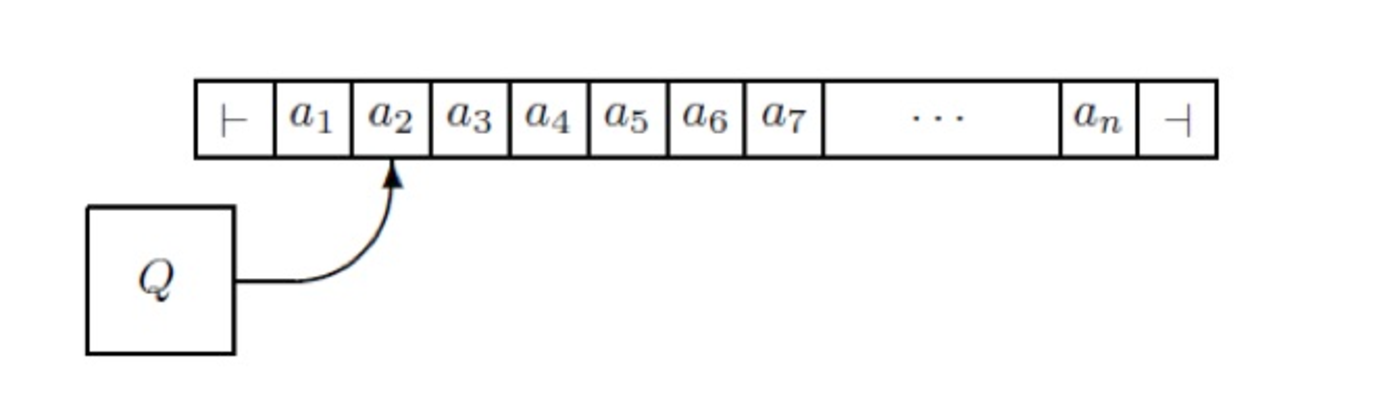
\includegraphics[width=0.65\textwidth]{Screenshot 2024-03-15 at 3.05.42 PM.pdf}
\begin{itemize}
  \item Two-way Finite Automata has a read head, which
can move left or right over the input string .
\item Read head can revisit the input symbols any number of times.
\item The input string is enclosed between left and right
endmarkers $\vdash$ and $\dashv$, which are not elements of the
input alphabet $\Sigma$.
\item The read head will not move outside of the
endmarkers.
\item A 2DFA needs only a single accept state and a single reject state.
\end{itemize}
\end{frame}

\begin{frame}{Turing Machine vs 2DFA}
  
    \textbf{Turing Machine:}
    \begin{itemize}
      \item Contains a \textcolor{violet}{read/write} head that moves left or right along the tape 
      \item Has \textcolor{violet}{unbounded} memory.
    \end{itemize}
    \hspace*{1cm}\\
    \textbf{2DFA:}
    \begin{itemize}
      \item Has  \textcolor{violet}{read} only head that moves left or right along the tape.
      \item Has \textcolor{violet}{finite} memeory like DFA.
    \end{itemize}
  
\end{frame}

\section{Formal Definitions, Notations and Construction}

\begin{frame}
\frametitle{Formal representation of 2DFA}

A \emph{2DFA} is of the form 
\textbf{\[(Q, \Sigma, \vdash, \dashv, \delta, s, t, r)\]}
where,
\begin{itemize}
\item $Q$ is a finite set of states.
\item $\Sigma$ is a finite set of input symbols.
\item $\vdash$ is the left endmarker. ($\vdash \notin \Sigma$)
\item $\dashv$ is the right endmarker. ($\dashv \notin \Sigma$)
\item $\delta : Q \times (\Sigma \cup \{\vdash, \dashv\}) \rightarrow Q \times \{L, R\}$ is a transition function. \\(L $=$ left, R $=$ right)
\item $s \in Q$ is the start state.
\item $t \in Q$ is the accept state.
\item $r \in Q$ is the reject state ($r \neq t$).
\end{itemize}
\end{frame}

\begin{frame}
\frametitle{Properties of transition function}

For all states $p$,
\begin{itemize}
\item \textcolor{red}{$\delta(p,\vdash) = (q,R)$}, for some $q \in Q$ 
\item \textcolor{red}{$\delta(p, \dashv) = (q, L)$}, for some $q \in Q $
\end{itemize}
\hspace*{1cm}\\
Current input symbol is $a \in \Sigma \cup \{\vdash\}$, $t =$ accept state, $r =$ reject state.
\begin{itemize}
\item \textcolor{red}{$\delta(t,a) = (t,R)$ and $\delta(t,\dashv) = (t,L)$} 
\item \textcolor{red}{$\delta(r,a) = (r,R)$ and $\delta(r,\dashv) = (r,L)$}
\end{itemize}
\hspace*{1cm}\\
 In general, $\delta(p,a) = (q,d)$ where $p,q \in Q$ and $d \in \{L,R\}$

\end{frame}

%\begin{frame}{Example 2DFA}
%\begin{exampleblock}{2DFA for $a^{*}$}
%\begin{tikzpicture}[shorten >=1pt,node distance=2.5cm,on grid,auto] 
%\node[state,initial] (q0) {$q_0$}; 
%\node[state,accepting] (q1) [right=of q0] {$q_1$};
%\node[state] (q2) [below=of q0] {$q_2$};
%\path[->] 
%(q0) edge [loop above] node {($a,R$),($\vdash, R$)} (q0)
 %       edge node {$\dashv,L$} (q1)
  %      edge node {$b,R$} (q2)
%(q1) edge [loop above] node {$a,R$} (q1)
 %        edge [loop right] node {$b,R$} (q1)
  %       edge [loop below] node {($\dashv,L$),($\vdash, R$)} (q1)
%(q2) edge [loop left] node {$a,R$} (q2)
 %        edge [loop below] node {$b,R$} (q2)
  %       edge [loop right] node {($\dashv,L$),($\vdash, R$)} (q2);
%\end{tikzpicture}
%\end{exampleblock}
%\end{frame}

\begin{frame}
\frametitle{Example 2DFA}
 \centering
        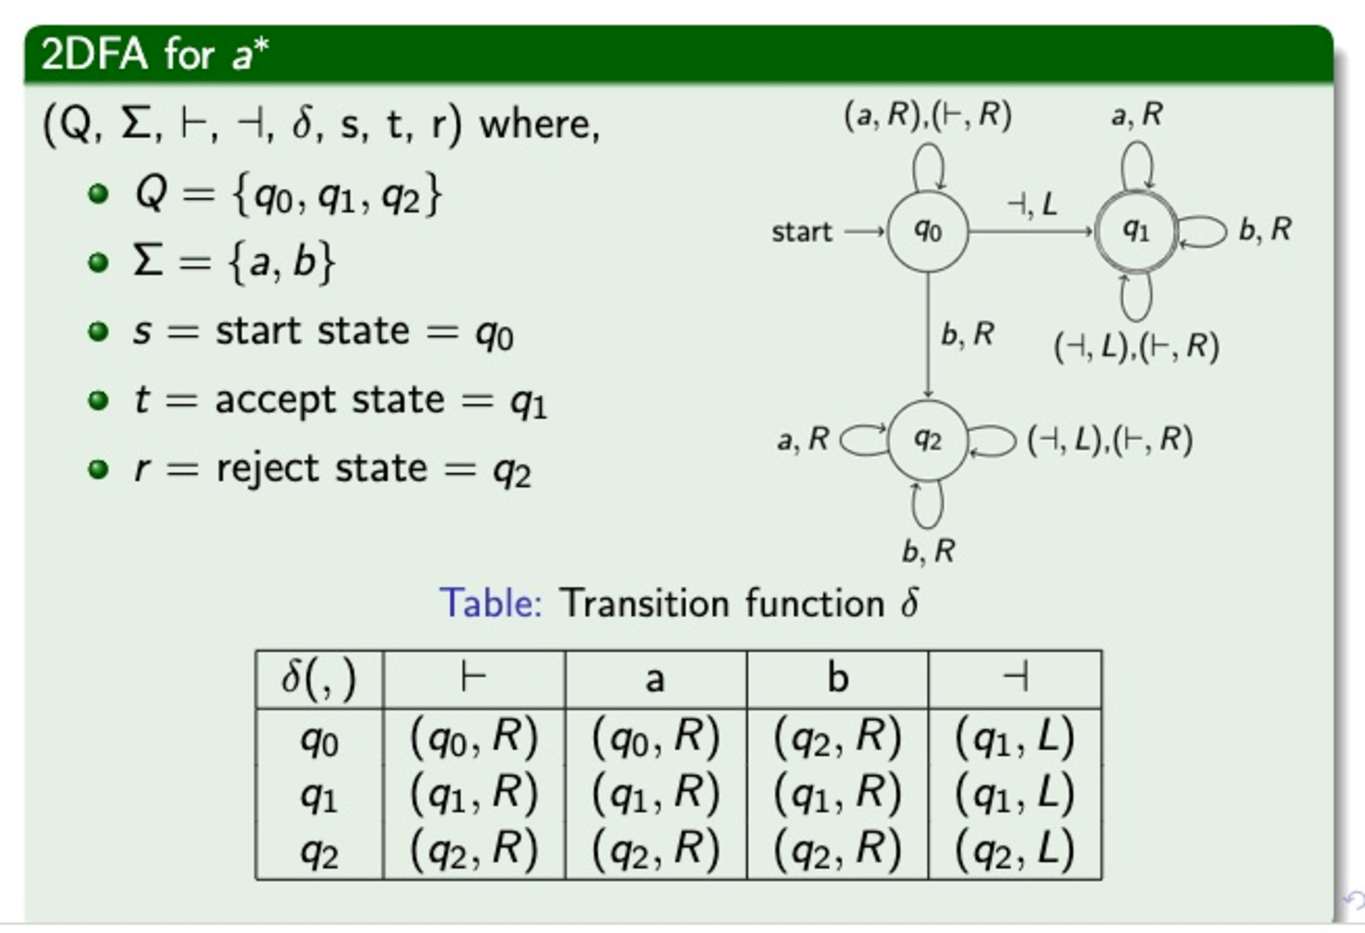
\includegraphics[width=1.0\textwidth]{Screenshot 2024-03-15 at 6.08.48 PM copy.pdf}
    
\end{frame}

\begin{frame}{Configurations }
Fix an input $x \in \Sigma^{*}$. $x = a_{1}a_{2}a_{3} \ldots a_{n}$. Let $a_{0} = \vdash$ and $a_{n+1} = \dashv$. \\
$a_0a_1a_2a_3 \ldots a_n a_{n+1} = \vdash x \dashv$. \\
\begin{block}{Configuration}
A configuration of the machine on input $x$ is a pair $(q, i)$ such that $q \in Q$ and $0 \leq i \leq n + 1$. Informally, the pair $(q, i)$ gives a \textcolor{red}{current state} and \textcolor{red}{current position} of the read head. \\
The \textcolor{red}{start configuration is $(s, 0)$}, meaning that the machine is in its start state $s$ and scanning the left endmarker.
\end{block}
A binary relation $\xrightarrow[x]{1}$, the next configuration relation, is defined on configurations as follows:
\[
\delta(p, a_i) = (q, L) \Rightarrow (p, i) \xrightarrow[x]{1} (q, i - 1),
\]
\[
\delta(p, a_i) = (q, R) \Rightarrow (p, i) \xrightarrow[x]{1} (q, i + 1).
\]
\end{frame}

\begin{frame}{Configurations }
The relation $\xrightarrow[x]{1}$ describes one step of the machine on input $x$. We define the relations $\xrightarrow[x]{n}$ inductively, $n \geq 0$:
\begin{itemize}
\item $(p, i) \xrightarrow[x]{0} (p, i)$
\item if $(p, i) \xrightarrow[x]{n}(q, j)$ and $(q, j) \xrightarrow[x]{1} (u, k)$, then $(p, i) \xrightarrow[x]{n+1} (u, k)$.
\end{itemize}
\hspace*{1cm}\\
For any configuration $(p, i)$, there is exactly one configuration $(q, j)$ such that $(p, i) \xrightarrow[x]{n} (q, j)$. \\


\end{frame}
\begin{frame}{Acceptance and Rejection}
  
    \hspace*{1cm}$(p,i) \xrightarrow[x]{*} (q,j)$ iff  $\exists$$n \geq 0$ such that $(p,i) \xrightarrow[x]{n} (q,j)$.
    
\begin{block}{Acceptance}
The input $x$ is accepted by the machine iff $(s, 0) \xrightarrow[x]{*} (t, k)$ for some k.
\end{block}
\begin{block}{Rejection}
  \begin{itemize}
\item The input $x$ is rejected by the machine if $(s, 0) \xrightarrow[x]{*} (r, k)$ for some k.
\end{itemize}
\end{block}

  
 If the machine neither reaches accept state nor reject state then the machine is said to be looping on that input.\\
 
Language accepted by the machine = $\{x \in \Sigma^{*} | x$ is accepted by the machine$\}$.

  \end{frame}


\begin{frame}{Constructing 2DFA 'M'}
  %length of a is divisible by 3 and length of b is divisible by 2
   $L(M) = \{x \in \Sigma^* \mid \#a(x)$ is multiple of 3, $\#b(x)$ is multiple of 2\}
  \begin{exampleblock}{Machine Description}
  \begin{itemize}
  \item Machine starts scanning from the left endmarker.
  \item Scan input string from left to right, counting only 'a's. If the count of 'a's is not a multiple of 3, reject and enter state $r$.\\
  \item Let $q_0,q_1,q_2$ be the states for counting 'a's. \\$q_0$: 3k; $q_1$: 3k+1; $q_2$: 3k+2.
  \item If the count of 'a's is a multiple of 3, start scanning from the right, counting only 'b's. If the count of 'b's is not a multiple of 2, enter state $t$; otherwise, enter state $r$.\\
  \item Let $p_0,p_1$ be the states for counting 'b's. \\$p_0$: 2k; $p_1$: 2k+1.
  \end{itemize}
  \end{exampleblock}
\end{frame}

\begin{frame}{Constructing 2DFA 'M'}
  %to check for few inputs and their acceptance 1.abba 2.bbaabab
  \centering
  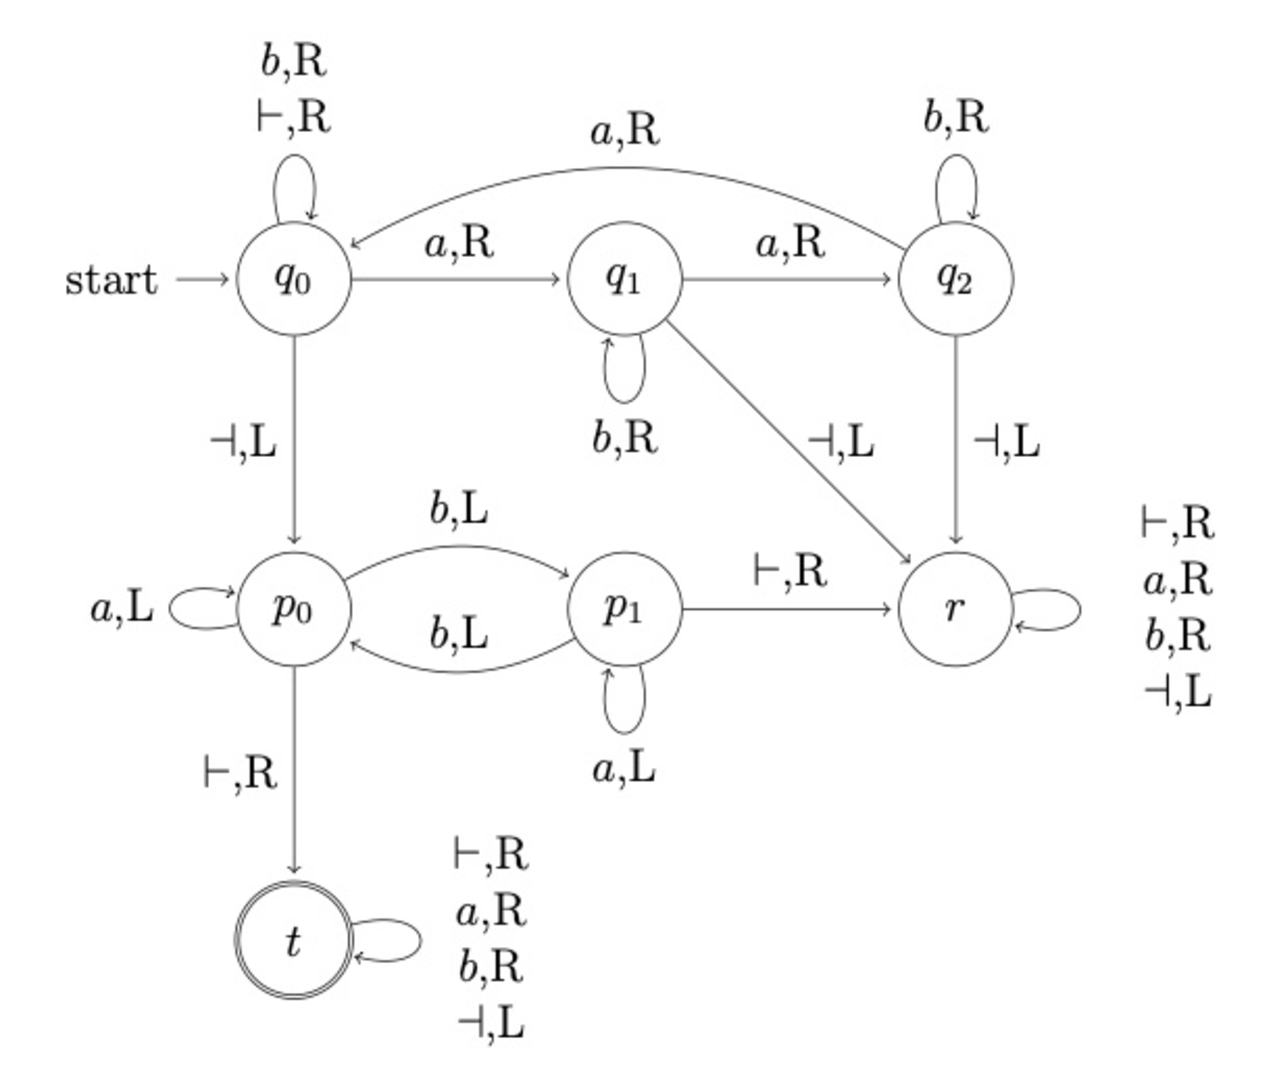
\includegraphics[width=0.6\textwidth]{Screenshot 2024-03-13 at 3.50.28 PM.pdf}
  \begin{itemize}
    
    \item input $=$ bbaabab :\\
    
       $ q_0 \xrightarrow{\vdash} q_0 \xrightarrow{b} q_0 \xrightarrow{b} q_0 \xrightarrow{a} q_1 \xrightarrow{a} q_2 \xrightarrow{b} q_2 \xrightarrow{a} q_0 \xrightarrow{b} q_0 \xrightarrow{\dashv} p_0 \xrightarrow{b} p_1 \xrightarrow {a} p_1 \xrightarrow{b} p_0 .....\xrightarrow{\dashv} t$\\
     
  \end{itemize}
\end{frame}

  \section{Languages accepted by 2DFA}
\begin{frame}{DFA to 2DFA conversion}
\begin{block}{Theorem}
  \begin{itemize}
  \item 2DFA only accepts regular languages.\\
  \item L(2DFA) = L(DFA) = Regular languages\\ 
  \end{itemize}
\end{block}

\begin{block}{Proof: L(DFA) $\subseteq$ L(2DFA)}
  For an arbitary DFA 'X', let us construct a 2DFA 'Y' that accepts the same language as X.\\
  
\begin{itemize}
  \item X : (Q, $\Sigma$, $\delta$, s, F)\\
  \item Let Y : (Q $\cup$ \{t, r\}, $\Sigma$, $\vdash$, $\dashv$, $\delta'$, s, t, r)\\
  %delta is defined as delta union transition from (final start in F , left end marker) to (t, L) and  (non final start i.e  Q-F , left end marker) to (r, L) and (s, right end marker ) to (s,R)
  \item $\delta'$: $\delta_R$ $\cup $ {\\
$\delta'$((s, $\vdash$)) = (s, R)\\
  $\delta'$((f, $\dashv$)) = (t, L) for f $\in$ F ;\hspace*{0.1cm} $\delta'$((n, $\dashv$)) = (r, L) for n $\in$ Q-F.\\
   $\delta'$((t, a)) = (t, R) ;\hspace*{0.3cm} $\delta'$((r, a)) = (r, R) for a $\in$ $\Sigma-\{\dashv\}$ }\\
   $\delta'$((t,$\dashv))$ = (t,L) ;\hspace*{0.5cm} $\delta'$((r,$\dashv))$ = (r,L)\\
    \end{itemize}
\end{block}
 
\end{frame}

\begin{frame}{DFA to 2DFA conversion}
  \begin{block}{Proof: L(X) $\subseteq$ L(Y)}
  \begin{itemize}
    \item Let x $\in$ L(X), len(x)=n. \\
    \item Then, $\deltahat$(s,x) = f where f $\in$ F \\
    \item (s,0) $\xrightarrow[\vdash x \dashv]{1}$ (s,1) $\xrightarrow[\vdash x \dashv]{n}$ (f,n+1) $\xrightarrow[\vdash x \dashv]{1}$ (t,n) .\\
    \item As (s,0) $\xrightarrow[\vdash x \dashv]{*}$ (t,n+1), x $\in$ L(Y).\\
    \item Hence, L(X) $\subseteq$ L(Y).\\
  \end{itemize}
  \end{block}
  Recall: \\
  A configuration of the machine on input $x$ is the pair \textcolor{blue}{$(q, i)$} , which gives the \textcolor{blue}{current state} and \textcolor{blue}{current position of the read head}. \\
  $(s, 0)$ means that the machine is in its start state $s$ and scanning the left endmarker.
  
\end{frame}

\begin{frame}{DFA to 2DFA conversion}
  \begin{block}{Proof: L(Y) $\subseteq$ L(X)}
  \begin{itemize}
    \item Let x $\in$ L(Y), len(x)=n. \\
    \item Then (s,0) $\xrightarrow[\vdash x \dashv]{*}$ (t,m) in Y\\
    \item So (s,0) $\xrightarrow[\vdash x \dashv]{1}$ (s,1) $\xrightarrow[\vdash x \dashv]{n}$ (f,n+1) $\xrightarrow[\vdash x \dashv]{1}$ (t,n) .\\
    \item As $\deltahat$(s,x) = f where f $\in$ F, x $\in$ L(X)\\
    
    \item Hence, L(Y) $\subseteq$ L(X).\\
  \end{itemize}
  \end{block}
   \textbf{Therefore, L(Y) = L(X)}
\end{frame}


\end{document}
